% Options for packages loaded elsewhere
\PassOptionsToPackage{unicode}{hyperref}
\PassOptionsToPackage{hyphens}{url}
\PassOptionsToPackage{dvipsnames,svgnames,x11names}{xcolor}
%
\documentclass[
  ignorenonframetext,
]{beamer}
\usepackage{pgfpages}
\setbeamertemplate{caption}[numbered]
\setbeamertemplate{caption label separator}{: }
\setbeamercolor{caption name}{fg=normal text.fg}
\beamertemplatenavigationsymbolsempty
% Prevent slide breaks in the middle of a paragraph
\widowpenalties 1 10000
\raggedbottom

\usepackage{amsmath,amssymb}
\usepackage{iftex}
\ifPDFTeX
  \usepackage[T1]{fontenc}
  \usepackage[utf8]{inputenc}
  \usepackage{textcomp} % provide euro and other symbols
\else % if luatex or xetex
  \usepackage{unicode-math}
  \defaultfontfeatures{Scale=MatchLowercase}
  \defaultfontfeatures[\rmfamily]{Ligatures=TeX,Scale=1}
\fi
\usepackage{lmodern}
\usetheme[]{AnnArbor}
\usecolortheme{dolphin}
\usefonttheme{structurebold}
\ifPDFTeX\else  
    % xetex/luatex font selection
\fi
% Use upquote if available, for straight quotes in verbatim environments
\IfFileExists{upquote.sty}{\usepackage{upquote}}{}
\IfFileExists{microtype.sty}{% use microtype if available
  \usepackage[]{microtype}
  \UseMicrotypeSet[protrusion]{basicmath} % disable protrusion for tt fonts
}{}
\makeatletter
\@ifundefined{KOMAClassName}{% if non-KOMA class
  \IfFileExists{parskip.sty}{%
    \usepackage{parskip}
  }{% else
    \setlength{\parindent}{0pt}
    \setlength{\parskip}{6pt plus 2pt minus 1pt}}
}{% if KOMA class
  \KOMAoptions{parskip=half}}
\makeatother
\usepackage{xcolor}
\newif\ifbibliography
\setlength{\emergencystretch}{3em} % prevent overfull lines
\setcounter{secnumdepth}{-\maxdimen} % remove section numbering

\usepackage{color}
\usepackage{fancyvrb}
\newcommand{\VerbBar}{|}
\newcommand{\VERB}{\Verb[commandchars=\\\{\}]}
\DefineVerbatimEnvironment{Highlighting}{Verbatim}{commandchars=\\\{\}}
% Add ',fontsize=\small' for more characters per line
\usepackage{framed}
\definecolor{shadecolor}{RGB}{241,243,245}
\newenvironment{Shaded}{\begin{snugshade}}{\end{snugshade}}
\newcommand{\AlertTok}[1]{\textcolor[rgb]{0.68,0.00,0.00}{#1}}
\newcommand{\AnnotationTok}[1]{\textcolor[rgb]{0.37,0.37,0.37}{#1}}
\newcommand{\AttributeTok}[1]{\textcolor[rgb]{0.40,0.45,0.13}{#1}}
\newcommand{\BaseNTok}[1]{\textcolor[rgb]{0.68,0.00,0.00}{#1}}
\newcommand{\BuiltInTok}[1]{\textcolor[rgb]{0.00,0.23,0.31}{#1}}
\newcommand{\CharTok}[1]{\textcolor[rgb]{0.13,0.47,0.30}{#1}}
\newcommand{\CommentTok}[1]{\textcolor[rgb]{0.37,0.37,0.37}{#1}}
\newcommand{\CommentVarTok}[1]{\textcolor[rgb]{0.37,0.37,0.37}{\textit{#1}}}
\newcommand{\ConstantTok}[1]{\textcolor[rgb]{0.56,0.35,0.01}{#1}}
\newcommand{\ControlFlowTok}[1]{\textcolor[rgb]{0.00,0.23,0.31}{\textbf{#1}}}
\newcommand{\DataTypeTok}[1]{\textcolor[rgb]{0.68,0.00,0.00}{#1}}
\newcommand{\DecValTok}[1]{\textcolor[rgb]{0.68,0.00,0.00}{#1}}
\newcommand{\DocumentationTok}[1]{\textcolor[rgb]{0.37,0.37,0.37}{\textit{#1}}}
\newcommand{\ErrorTok}[1]{\textcolor[rgb]{0.68,0.00,0.00}{#1}}
\newcommand{\ExtensionTok}[1]{\textcolor[rgb]{0.00,0.23,0.31}{#1}}
\newcommand{\FloatTok}[1]{\textcolor[rgb]{0.68,0.00,0.00}{#1}}
\newcommand{\FunctionTok}[1]{\textcolor[rgb]{0.28,0.35,0.67}{#1}}
\newcommand{\ImportTok}[1]{\textcolor[rgb]{0.00,0.46,0.62}{#1}}
\newcommand{\InformationTok}[1]{\textcolor[rgb]{0.37,0.37,0.37}{#1}}
\newcommand{\KeywordTok}[1]{\textcolor[rgb]{0.00,0.23,0.31}{\textbf{#1}}}
\newcommand{\NormalTok}[1]{\textcolor[rgb]{0.00,0.23,0.31}{#1}}
\newcommand{\OperatorTok}[1]{\textcolor[rgb]{0.37,0.37,0.37}{#1}}
\newcommand{\OtherTok}[1]{\textcolor[rgb]{0.00,0.23,0.31}{#1}}
\newcommand{\PreprocessorTok}[1]{\textcolor[rgb]{0.68,0.00,0.00}{#1}}
\newcommand{\RegionMarkerTok}[1]{\textcolor[rgb]{0.00,0.23,0.31}{#1}}
\newcommand{\SpecialCharTok}[1]{\textcolor[rgb]{0.37,0.37,0.37}{#1}}
\newcommand{\SpecialStringTok}[1]{\textcolor[rgb]{0.13,0.47,0.30}{#1}}
\newcommand{\StringTok}[1]{\textcolor[rgb]{0.13,0.47,0.30}{#1}}
\newcommand{\VariableTok}[1]{\textcolor[rgb]{0.07,0.07,0.07}{#1}}
\newcommand{\VerbatimStringTok}[1]{\textcolor[rgb]{0.13,0.47,0.30}{#1}}
\newcommand{\WarningTok}[1]{\textcolor[rgb]{0.37,0.37,0.37}{\textit{#1}}}

\providecommand{\tightlist}{%
  \setlength{\itemsep}{0pt}\setlength{\parskip}{0pt}}\usepackage{longtable,booktabs,array}
\usepackage{calc} % for calculating minipage widths
\usepackage{caption}
% Make caption package work with longtable
\makeatletter
\def\fnum@table{\tablename~\thetable}
\makeatother
\usepackage{graphicx}
\makeatletter
\def\maxwidth{\ifdim\Gin@nat@width>\linewidth\linewidth\else\Gin@nat@width\fi}
\def\maxheight{\ifdim\Gin@nat@height>\textheight\textheight\else\Gin@nat@height\fi}
\makeatother
% Scale images if necessary, so that they will not overflow the page
% margins by default, and it is still possible to overwrite the defaults
% using explicit options in \includegraphics[width, height, ...]{}
\setkeys{Gin}{width=\maxwidth,height=\maxheight,keepaspectratio}
% Set default figure placement to htbp
\makeatletter
\def\fps@figure{htbp}
\makeatother
% definitions for citeproc citations
\NewDocumentCommand\citeproctext{}{}
\NewDocumentCommand\citeproc{mm}{%
  \begingroup\def\citeproctext{#2}\cite{#1}\endgroup}
\makeatletter
 % allow citations to break across lines
 \let\@cite@ofmt\@firstofone
 % avoid brackets around text for \cite:
 \def\@biblabel#1{}
 \def\@cite#1#2{{#1\if@tempswa , #2\fi}}
\makeatother
\newlength{\cslhangindent}
\setlength{\cslhangindent}{1.5em}
\newlength{\csllabelwidth}
\setlength{\csllabelwidth}{3em}
\newenvironment{CSLReferences}[2] % #1 hanging-indent, #2 entry-spacing
 {\begin{list}{}{%
  \setlength{\itemindent}{0pt}
  \setlength{\leftmargin}{0pt}
  \setlength{\parsep}{0pt}
  % turn on hanging indent if param 1 is 1
  \ifodd #1
   \setlength{\leftmargin}{\cslhangindent}
   \setlength{\itemindent}{-1\cslhangindent}
  \fi
  % set entry spacing
  \setlength{\itemsep}{#2\baselineskip}}}
 {\end{list}}
\usepackage{calc}
\newcommand{\CSLBlock}[1]{\hfill\break\parbox[t]{\linewidth}{\strut\ignorespaces#1\strut}}
\newcommand{\CSLLeftMargin}[1]{\parbox[t]{\csllabelwidth}{\strut#1\strut}}
\newcommand{\CSLRightInline}[1]{\parbox[t]{\linewidth - \csllabelwidth}{\strut#1\strut}}
\newcommand{\CSLIndent}[1]{\hspace{\cslhangindent}#1}


% logo
\titlegraphic{
\includegraphics[width=4cm]{../000_logos/logo-blue-vertical}}
\logo{\ifnum\thepage>1
\includegraphics[width=0.5cm]{../000_logos/logo-blue-vertical}\fi}

% UMNG: Manual de image institucional

% Colors

% Umng
\definecolor{yellow}{HTML}{fdc600}
\definecolor{red}{HTML}{ee2a24}

% Estudios a Distancia
\definecolor{blue1}{HTML}{12245b}
\definecolor{blue2}{HTML}{767ca6}
\definecolor{blue3}{HTML}{cad2ec}

% Modify items
\setbeamercolor{palette primary}{bg=blue3}
\setbeamercolor{palette tertiary}{bg=blue1}
\setbeamercolor{frametitle}{bg=yellow}

% Hyperlinks
\hypersetup{
  linkcolor=red,
  citecolor=red
}

\makeatletter
\@ifpackageloaded{caption}{}{\usepackage{caption}}
\AtBeginDocument{%
\ifdefined\contentsname
  \renewcommand*\contentsname{Table of contents}
\else
  \newcommand\contentsname{Table of contents}
\fi
\ifdefined\listfigurename
  \renewcommand*\listfigurename{List of Figures}
\else
  \newcommand\listfigurename{List of Figures}
\fi
\ifdefined\listtablename
  \renewcommand*\listtablename{List of Tables}
\else
  \newcommand\listtablename{List of Tables}
\fi
\ifdefined\figurename
  \renewcommand*\figurename{Figure}
\else
  \newcommand\figurename{Figure}
\fi
\ifdefined\tablename
  \renewcommand*\tablename{Table}
\else
  \newcommand\tablename{Table}
\fi
}
\@ifpackageloaded{float}{}{\usepackage{float}}
\floatstyle{ruled}
\@ifundefined{c@chapter}{\newfloat{codelisting}{h}{lop}}{\newfloat{codelisting}{h}{lop}[chapter]}
\floatname{codelisting}{Listing}
\newcommand*\listoflistings{\listof{codelisting}{List of Listings}}
\makeatother
\makeatletter
\makeatother
\makeatletter
\@ifpackageloaded{caption}{}{\usepackage{caption}}
\@ifpackageloaded{subcaption}{}{\usepackage{subcaption}}
\makeatother

\ifLuaTeX
\usepackage[bidi=basic]{babel}
\else
\usepackage[bidi=default]{babel}
\fi
\babelprovide[main,import]{english}
% get rid of language-specific shorthands (see #6817):
\let\LanguageShortHands\languageshorthands
\def\languageshorthands#1{}
\ifLuaTeX
  \usepackage{selnolig}  % disable illegal ligatures
\fi
\usepackage{bookmark}

\IfFileExists{xurl.sty}{\usepackage{xurl}}{} % add URL line breaks if available
\urlstyle{same} % disable monospaced font for URLs
\hypersetup{
  pdftitle={Welcome to R},
  pdfauthor={Luis Francisco Gómez López},
  pdflang={en},
  colorlinks=true,
  linkcolor={Maroon},
  filecolor={Maroon},
  citecolor={Blue},
  urlcolor={Blue},
  pdfcreator={LaTeX via pandoc}}


\title{Welcome to R}
\author{Luis Francisco Gómez López}
\date{2024-07-30}
\institute{FAEDIS}

\begin{document}
\frame{\titlepage}

\renewcommand*\contentsname{Table of contents}
\begin{frame}[allowframebreaks]
  \frametitle{Table of contents}
  \tableofcontents[hideallsubsections]
\end{frame}

\section{Please Read Me}\label{please-read-me}

\begin{frame}{}
\phantomsection\label{section}
\begin{itemize}
\tightlist
\item
  This presentation is based on (\citeproc{ref-chapman_r_2019}{Chapman
  and Feit 2019, chap. 1})
\end{itemize}
\end{frame}

\section{Purpose}\label{purpose}

\begin{frame}{}
\phantomsection\label{section-1}
\begin{itemize}
\tightlist
\item
  Deliver essential knowledge within a minimal timeframe by employing
  hands-on learning techniques to enhance productivity in the R
  programming language
\end{itemize}
\end{frame}

\section{Forgetting curves}\label{forgetting-curves}

\begin{frame}{}
\phantomsection\label{section-2}
\begin{itemize}
\tightlist
\item
  \textbf{Learning and forgetting curves}
  (\citeproc{ref-posit_pbc_learning_2023}{PBC 2023})
\end{itemize}

\begin{figure}[H]

{\centering 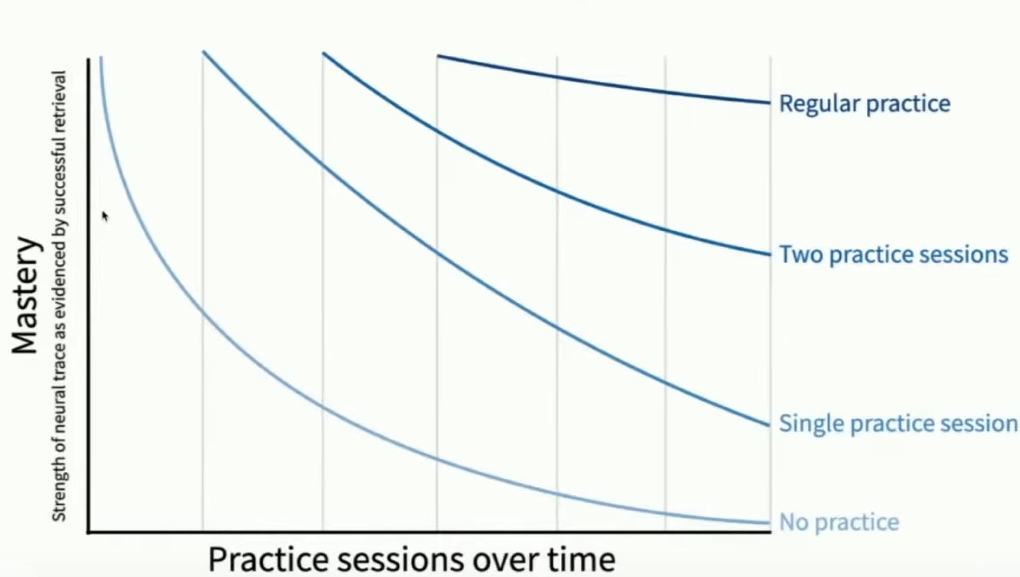
\includegraphics[width=3.64583in,height=3.64583in]{../000_images/002_forgetting_curves.png}

}

\caption{Learning and forgetting curves}

\end{figure}%
\end{frame}

\begin{frame}{}
\phantomsection\label{section-3}
\begin{itemize}
\tightlist
\item
  \textbf{Practicing and forgetting curves}
  (\citeproc{ref-posit_pbc_learning_2023}{PBC 2023})
\end{itemize}

\begin{figure}[H]

{\centering 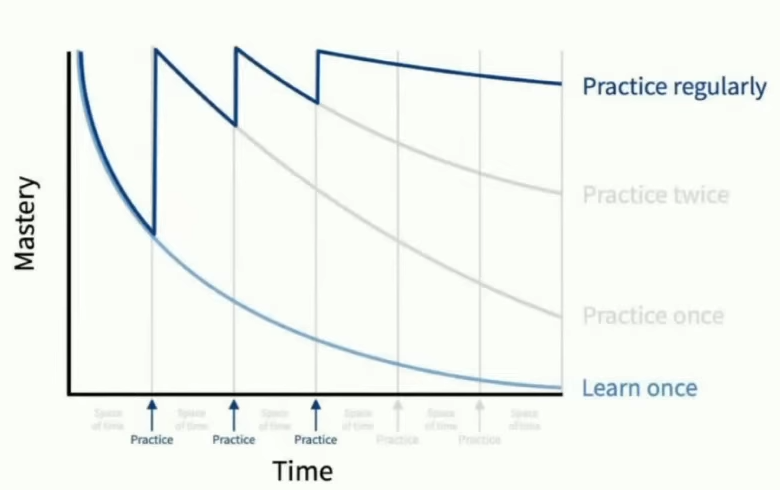
\includegraphics[width=3.64583in,height=3.64583in]{../000_images/002_forgetting_curves_practice.png}

}

\caption{Practicing and forgetting curves}

\end{figure}%
\end{frame}

\section{Installing R, RStudio IDE and
Quarto}\label{installing-r-rstudio-ide-and-quarto}

\begin{frame}{}
\phantomsection\label{section-4}
\begin{itemize}
\tightlist
\item
  \textbf{What are R and RStudio IDE?}
  (\citeproc{ref-ismay_statistical_2020}{Ismay and Kim 2020, chap. 1})
\end{itemize}

\begin{figure}

\begin{minipage}{0.50\linewidth}

\centering{

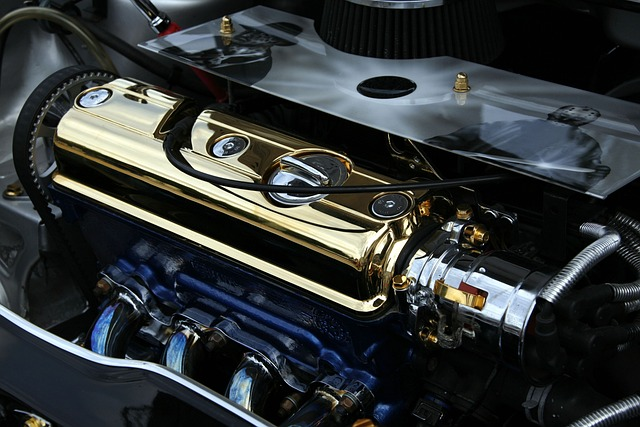
\includegraphics[width=2.08333in,height=2.08333in]{../000_images/002_car_engine.jpg}

}

\subcaption{\label{fig-r-1}R: Engine}

\end{minipage}%
%
\begin{minipage}{0.50\linewidth}

\centering{

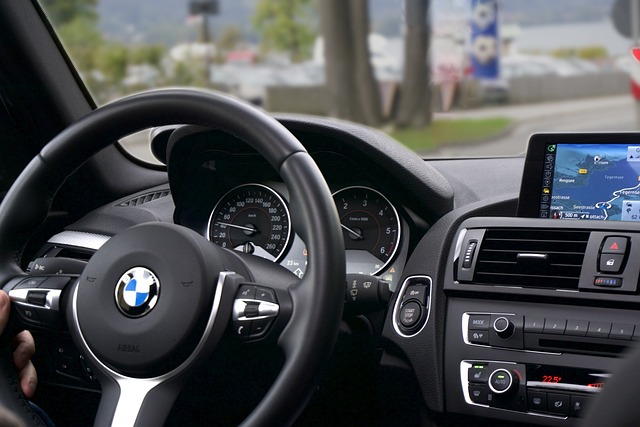
\includegraphics[width=2.08333in,height=2.08333in]{../000_images/002_dashboard_car.jpg}

}

\subcaption{\label{fig-rstudio-ide-1}RStudio IDE: Dashboard}

\end{minipage}%

\caption{\label{fig-r_vs_rstudio_ide_1}Analogy of difference between R
and RStudio}

\end{figure}%
\end{frame}

\begin{frame}{}
\phantomsection\label{section-5}
\begin{itemize}
\item
  \textbf{What is Quarto?}

  \begin{itemize}
  \tightlist
  \item
    Open-source scientific and technical publishing system
  \item
    It is possible to integrate prose, code and results via Rstudio IDE
    (\citeproc{ref-wickham_r_2023}{Wickham, Çetinkaya-Rundel, and
    Grolemund 2023, chap. 29})
  \end{itemize}
\end{itemize}

\begin{figure}

\centering{


\includegraphics[width=4.16667in,height=4.16667in]{../000_images/002_quarto_flow.png}

}

\caption{\label{fig-quarto}Quarto workflow}

\end{figure}%
\end{frame}

\begin{frame}{}
\phantomsection\label{section-6}
\begin{itemize}
\item
  \textbf{Download and install R}: \url{https://cloud.r-project.org/}

  \begin{itemize}
  \tightlist
  \item
    Download R for Linux (Debian, Fedora/Redhat, Ubuntu)
  \item
    Download R for macOS
  \item
    Download R for Windows
  \end{itemize}
\item
  \textbf{Download and install RStudio IDE}:
  \url{https://posit.co/download/rstudio-desktop/}

  \begin{itemize}
  \tightlist
  \item
    Windows 10/11
  \item
    macOS 11+
  \item
    Ubuntu 18/Debian 10, Ubuntu 20/Debian 11, Ubuntu 22, Fedora 19/Red
    Hat 7, OpenSUSE 15, Fedora 34/Red Hat 8, Fedora 36/Red Hat 9
  \end{itemize}
\end{itemize}
\end{frame}

\begin{frame}{}
\phantomsection\label{section-7}
\begin{itemize}
\item
  \textbf{Download and install Quarto}:
  \url{https://quarto.org/docs/get-started/}

  \begin{itemize}
  \tightlist
  \item
    Ubuntu 18+/Debian 10+, Linux Arm64
  \item
    Mac OS
  \item
    Windows
  \end{itemize}
\item
  \textbf{Nothing works help me!!!}

  \begin{itemize}
  \item
    Don't worry posit get you cover!!!
  \item
    Use posit Cloud: \url{https://posit.cloud/}

    \begin{itemize}
    \tightlist
    \item
      Sign Up \textgreater{} Cloud Free \textgreater{} Sign Up
    \end{itemize}
  \end{itemize}
\end{itemize}
\end{frame}

\begin{frame}{}
\phantomsection\label{section-8}
\begin{itemize}
\item
  \textbf{Using R and Quarto via RStudio IDE}
  (\citeproc{ref-ismay_statistical_2020}{Ismay and Kim 2020, chap. 1})

  \begin{itemize}
  \tightlist
  \item
    Don't worry about Quarto because it will be embedded in RStudio IDE

    \begin{itemize}
    \tightlist
    \item
      If you are using posit Cloud don't worry about anything!!!
    \end{itemize}
  \end{itemize}
\end{itemize}

\begin{figure}

\begin{minipage}{0.50\linewidth}

\centering{


\includegraphics[width=1.04167in,height=1.04167in]{../000_images/002_R_logo.png}

}

\subcaption{\label{fig-r-2}R: Do not open this}

\end{minipage}%
%
\begin{minipage}{0.50\linewidth}

\centering{


\includegraphics[width=0.83333in,height=0.83333in]{../000_images/002_RStudio_ide_logo.png}

}

\subcaption{\label{fig-rstudio-ide-2}RStudio IDE: Open this}

\end{minipage}%

\caption{\label{fig-r_vs_rstudio_ide_2}R versus RStudio IDE icons on
your computer}

\end{figure}%
\end{frame}

\section{R packages}\label{r-packages}

\begin{frame}{}
\phantomsection\label{section-9}
\begin{itemize}
\tightlist
\item
  \textbf{What are R packages?}
  (\citeproc{ref-ismay_statistical_2020}{Ismay and Kim 2020, chap. 1})
\end{itemize}

\begin{figure}

\begin{minipage}{0.50\linewidth}

\centering{

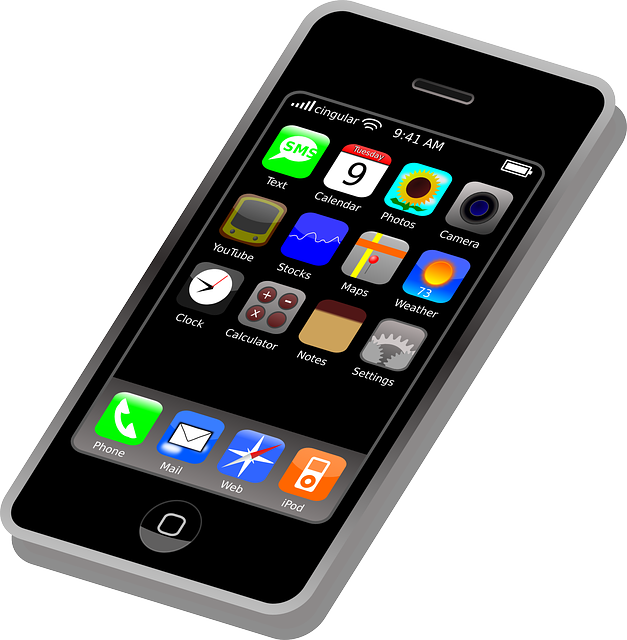
\includegraphics[width=1.04167in,height=1.04167in]{../000_images/002_cell_phone.png}

}

\subcaption{\label{fig-package-base}R: A new phone}

\end{minipage}%
%
\begin{minipage}{0.50\linewidth}

\centering{


\includegraphics[width=1.45833in,height=0.83333in]{../000_images/002_apps.jpg}

}

\subcaption{\label{fig-package}R packages: Apps you can download}

\end{minipage}%

\caption{\label{fig-r_packages}Analogy of R vs R packages}

\end{figure}%
\end{frame}

\begin{frame}[fragile]{}
\phantomsection\label{section-10}
\begin{itemize}
\item
  \textbf{Installing the tidyverse as an example}

  \begin{itemize}
  \item
    Copy and paste this code in the console. If you have already
    installed the tidyverse nothing will happen but if you don't have
    installed the tidyverse then the package is going to be installed
  \item
    Installing a package is like downloading an app from a store where
    you need to do it only once
  \end{itemize}
\end{itemize}

\tiny

\begin{Shaded}
\begin{Highlighting}[]
\NormalTok{packages }\OtherTok{\textless{}{-}} \FunctionTok{c}\NormalTok{(}\StringTok{"tidyverse"}\NormalTok{)}
\ControlFlowTok{for}\NormalTok{ (package }\ControlFlowTok{in}\NormalTok{ packages) \{}
  \ControlFlowTok{if}\NormalTok{ (}\SpecialCharTok{!}\NormalTok{(package }\SpecialCharTok{\%in\%} \FunctionTok{rownames}\NormalTok{(}\FunctionTok{installed.packages}\NormalTok{()))) \{}
    \FunctionTok{install.packages}\NormalTok{(package)}
\NormalTok{  \}}
\NormalTok{\}}
\end{Highlighting}
\end{Shaded}

\normalsize

\begin{itemize}
\item
  \textbf{Loading a package}

  \begin{itemize}
  \tightlist
  \item
    Loading a package is like opening an app you already installed on
    your phone where you need to do it every time you want to use the
    app
  \end{itemize}
\end{itemize}

\tiny

\begin{Shaded}
\begin{Highlighting}[]
\FunctionTok{library}\NormalTok{(tidyverse)}
\end{Highlighting}
\end{Shaded}
\end{frame}

\section{Please help me: Errors, warnings, and
messages}\label{please-help-me-errors-warnings-and-messages}

\begin{frame}[fragile]{}
\phantomsection\label{section-11}
\begin{itemize}
\tightlist
\item
  \textbf{Error}: Generally when there's an error, the code will not run
  and a message will try to explain what went wrong
  (\citeproc{ref-ismay_statistical_2020}{Ismay and Kim 2020, chap. 1})
\end{itemize}

\tiny

\begin{Shaded}
\begin{Highlighting}[]
\NormalTok{x }\OtherTok{\textless{}{-}} \FunctionTok{c}\NormalTok{(}\DecValTok{1}\NormalTok{, }\DecValTok{2}\NormalTok{, }\DecValTok{3}\NormalTok{, }\DecValTok{4}\NormalTok{, }\DecValTok{5}\NormalTok{)}
\NormalTok{X}
\end{Highlighting}
\end{Shaded}

\begin{verbatim}
Error in eval(expr, envir, enclos): object 'X' not found
\end{verbatim}

\normalsize

\begin{itemize}
\tightlist
\item
  \textbf{Warning}: Generally your code will still work, but with some
  caveats (\citeproc{ref-ismay_statistical_2020}{Ismay and Kim 2020,
  chap. 1})
\end{itemize}

\tiny

\begin{Shaded}
\begin{Highlighting}[]
\FunctionTok{sqrt}\NormalTok{(}\SpecialCharTok{{-}}\DecValTok{9}\NormalTok{)}
\end{Highlighting}
\end{Shaded}

\begin{verbatim}
Warning in sqrt(-9): NaNs produced
\end{verbatim}

\begin{verbatim}
[1] NaN
\end{verbatim}
\end{frame}

\begin{frame}[fragile]{}
\phantomsection\label{section-12}
\normalsize

\begin{itemize}
\item
  \textbf{Message}: it's just a friendly message
  (\citeproc{ref-ismay_statistical_2020}{Ismay and Kim 2020, chap. 1})

  \begin{itemize}
  \tightlist
  \item
    Read it, wave back at R, and thank it for talking to you
    (\citeproc{ref-ismay_statistical_2020}{Ismay and Kim 2020, chap. 1})
  \end{itemize}
\end{itemize}

\tiny

\begin{Shaded}
\begin{Highlighting}[]
\NormalTok{packages}\OtherTok{\textless{}{-}}\FunctionTok{c}\NormalTok{(}\StringTok{"tidyverse"}\NormalTok{)}
\ControlFlowTok{for}\NormalTok{(package }\ControlFlowTok{in}\NormalTok{ packages) \{}
  \ControlFlowTok{if}\NormalTok{(}\SpecialCharTok{!}\NormalTok{(package }\SpecialCharTok{\%in\%} \FunctionTok{rownames}\NormalTok{(}\FunctionTok{installed.packages}\NormalTok{()))) \{}
    \FunctionTok{install.packages}\NormalTok{(package)}
\NormalTok{  \}}
\NormalTok{\}}
\FunctionTok{library}\NormalTok{(tidyverse)}
\end{Highlighting}
\end{Shaded}

\begin{verbatim}
-- Attaching core tidyverse packages ------------------------ tidyverse 2.0.0 --
v dplyr     1.1.4     v readr     2.1.5
v forcats   1.0.0     v stringr   1.5.1
v ggplot2   3.5.1     v tibble    3.2.1
v lubridate 1.9.3     v tidyr     1.3.1
v purrr     1.0.2     
-- Conflicts ------------------------------------------ tidyverse_conflicts() --
x dplyr::filter() masks stats::filter()
x dplyr::lag()    masks stats::lag()
i Use the conflicted package (<http://conflicted.r-lib.org/>) to force all conflicts to become errors
\end{verbatim}
\end{frame}

\section{R for Marketing Research and Analytics, 2nd
Ed}\label{r-for-marketing-research-and-analytics-2nd-ed}

\begin{frame}{}
\phantomsection\label{section-13}
\begin{itemize}
\item
  \textbf{Download from UMNG Springer Link database}:

  \begin{itemize}
  \tightlist
  \item
    \url{https://doi-org.ezproxy.umng.edu.co/10.1007/978-3-030-14316-9}
  \end{itemize}
\item
  \textbf{Check the book site}:

  \begin{itemize}
  \tightlist
  \item
    \url{http://r-marketing.r-forge.r-project.org}
  \end{itemize}
\end{itemize}
\end{frame}

\section{Acknowledgments}\label{acknowledgments}

\begin{frame}{}
\phantomsection\label{section-14}
\begin{itemize}
\item
  To my family that supports me
\item
  To the taxpayers of Colombia and the
  \href{https://www.umng.edu.co/estudiante}{\textbf{UMNG students}} who
  pay my salary
\item
  To the \href{https://www.business-science.io/}{\textbf{Business
  Science}} and \href{https://www.rfordatasci.com/}{\textbf{R4DS Online
  Learning}} communities where I learn
  \href{https://www.r-project.org/about.html}{\textbf{R}} and
  \href{https://www.python.org/about/}{\textbf{\(\pi\)-thon}}
\item
  To the \href{https://www.r-project.org/contributors.html}{\textbf{R
  Core Team}}, the creators of
  \href{https://posit.co/products/open-source/rstudio/}{\textbf{RStudio
  IDE}}, \href{https://quarto.org/}{\textbf{Quarto}} and the authors and
  maintainers of the packages
  \href{https://CRAN.R-project.org/package=tidyverse}{\textbf{tidyverse}}
  and
  \href{https://CRAN.R-project.org/package=tinytex}{\textbf{tinytex}}
  for allowing me to access these tools without paying for a license
\item
  To the \href{https://www.kernel.org/category/about.html}{\textbf{Linux
  kernel community}} for allowing me the possibility to use some
  \href{https://static.lwn.net/Distributions/}{\textbf{Linux
  distributions}} as my main
  \href{https://en.wikipedia.org/wiki/Operating_system}{\textbf{OS}}
  without paying for a license
\end{itemize}
\end{frame}

\section*{References}\label{references}
\addcontentsline{toc}{section}{References}

\begin{frame}[allowframebreaks]{References}
\phantomsection\label{refs}
\begin{CSLReferences}{1}{0}
\bibitem[\citeproctext]{ref-chapman_r_2019}
Chapman, Chris, and Elea McDonnell Feit. 2019. \emph{R {For} {Marketing}
{Research} and {Analytics}}. 2nd ed. 2019. Use {R}! Cham: Springer
International Publishing : Imprint: Springer.
\url{https://doi.org/10.1007/978-3-030-14316-9}.

\bibitem[\citeproctext]{ref-ismay_statistical_2020}
Ismay, Chester, and Albert Young-Sun Kim. 2020. \emph{Statistical
Inference via Data Science: A {ModernDive} into {R} and the Tidyverse}.
The {R} Series. Boca Raton London New York: CRC Press, Taylor \& Francis
Group. \url{https://moderndive.com/index.html}.

\bibitem[\citeproctext]{ref-posit_pbc_learning_2023}
PBC, Posit. 2023. {``Learning {Python} for {Data} {Science} with {Posit}
{Academy} - {YouTube}.''}
\url{https://www.youtube.com/live/IpUhSZPqTaE?feature=share&t=401}.

\bibitem[\citeproctext]{ref-wickham_r_2023}
Wickham, Hadley, Mine Çetinkaya-Rundel, and Garret Grolemund. 2023. {``R
for {Data} {Science} (2e).''} \url{https://r4ds.hadley.nz/}.

\end{CSLReferences}
\end{frame}




\end{document}
